%!TEX root = ../CombinatoricsNotes.tex

 \section{Representing Sets and Sperner Systems.}
 \lect{1}{11}
% \marginnote{Lecture 2: Monday, January 11, 2016. }
\marginnote{We begin our systematic investigation into extremal combinatorics.}
Let's start with some definitions. 
\begin{itemize}[]
\item[Power set:] 
Let $X$ be a finite set with cardinality $|X| = n$. The \defn{power set} is $\P(X)$, the collection of subsets of $X$. $|\P(X)|= 2^n$.
\item[$r$-element subsets:] 
The set $X^{(r)}$ is the collection of all $r$-element subsets of $X$. The cardinality $|X^{(r)}| = {n\choose r}$.
\item[Set system:]
A \defn{set system} $\F \subset \P(X)$ on $X$ is a collection of subsets of $X$. For example, $\F = \{\emptyset, \{1\}, \{1,2\}, \{2,3\},\{3\}\}$ is a set system on $\{1,2,3\}$.
\item[$r$-graph:]
If $\F\subset X^{(r)}$, then we call $\F$ an $r$-graph or \defn{hypergraph}. 2-graphs are just ordinary graphs: $\F\subset X^{(2)}$ can be thought of as a graph with vertex set $X$, edge set $\F$.
\end{itemize}
We'll also frequently use the notation $[n] = \{1,2,\dotsc,n\}$.

\newthought{Now, given a set system} $\{A_1,A_2,\dotsc,A_m\}$, we want to ``reduce'' the sets such that distinct sets remain distinct.
That is, we want to find $S\subset X$ as small as possible such that $\{A_1\cap S, A_2\cap S, \dotsc, A_m\cap S\}$ are all distinct. \marginnote{Note that $S$ acts by deleting elements from our base set $X$.}
Let's start with two sets, $\{A_1,A_2\}$. We want $S$ as small as possible such that $A_1\cap S\neq A_2\cap S$. In this case, we can simply choose $S$ to be a singleton of an element which is in one set but not the other\sidenote{which always exists because $A_1\neq A_2$.}.
If we use our example earlier, $\{\emptyset, \{1\}, \{1,2\}, \{2,3\},\{3\}\}$ on $[3]$, we cannot remove any; $|\P([2])| = 4$ and we have five elements.
If our set system is $\{\emptyset, \{1,2\}, \{2,3\},\{3\}\}$ on $[3]$, then we may remove $1$; that is, $S = \{2,3\}$.
This motivates a question: How small can $S$ be as a function of $m$?
\begin{theorem}
Let $\F = \{A_1,A_2,\dotsc,A_m\}$ be a set system. Then there exists $S$, $|S|\leq m-1$ such that $A_1\cap S$, $A_2\cap S$, \ldots, $A_m\cap S$ are all distinct.
\end{theorem}
\begin{remark}
The bound is tight: the set system $\{\emptyset, \{1\}, \{2\}, \dotsc, \{m-1\}\}$ has the property that if we remove any element, we collapse two sets to the empty set.
\end{remark}
\begin{proof}	
Choose $S$ as small as possible such that $A_1\cap S$, $A_2\cap S$, \ldots, $A_m\cap S$ are all distinct, and assume that $|S| \geq m$.
Let $A_i' = A_i\cap S$. By the minimality of $S$ for every $x\in S$ there exists $i,j\in[m]$ such that $A_i'\setminus \{x\} = A_j'\setminus \{x\}$, with $i\neq j$.

Now, construct a graph  on the vertex set $[m]$ as follows. For each $x\in S$, choose one pair $i$ and $j$ ($i\neq j$) such that $A_i'\setminus \{x\} = A_j'\setminus \{x\}$, and join $i$ and $j$ by an edge\sidenote[][-2cm]{$A_i'\setminus \{x\} = A_j'\setminus \{x\}$ is equivalent to $A_i \symd A_j  =\{x\}$, where the symmetric difference $X\symd Y = (X\cup Y)\setminus (X\cap Y)$.
Because of this, we will make a new edge each time: if $x,y\in S$ yielded the same edge, then $\{x\}=A_i \symd A_j = \{y\} $.}. 
This graph has $m$ verticies and $|S|\geq m$ edges, so it contains a cycle\sidenote{Easy to see by picture; draw $m-1$ edges on $m$ vertices, and then if you don't have a cycle yet, you have a line, and no matter how you place the last edge, you get a cycle.}. Without loss of generality, assume there is a cycle on verticies $1,2,\dotsc,k$ in order. Then there exists distinct $x_1,x_2,\dotsc,x_k\in S$ such that $A_1\symd A_2 = \{x_1\}$, $A_2\symd A_3 = \{x_2\}$, \ldots, $A_{k-1}\symd A_k = \{x_{k-1}\}$, and $A_k \symd A_1 = \{x_k\}$. 

We can take the symmetric difference of all of them:
\[
\emptyset = (A_1\symd A_2) \symd (A_2 \symd A_3) \symd \dotsm \symd (A_k \symd A_1) = \{x_1,x_2,\dotsc, x_k\}
\]
\marginnote{Note the symmetric difference is commutative and associative.}
On the left, we have two of each set, so we can regroup and commute to obtain the empty set, using $A\symd A = \emptyset$. On the right, we have the symmetric difference of distinct singletons, which is just the union. This is a contradiction, so our minimal $S$ must have $|S|\leq m-1$.
\end{proof}
Before we continue finding ways to represent sets, we'll need some graph theoretic tools. First, some definitions.
% \begin{definition}
\begin{itemize}[]
	\item[Bipartite:]  
A graph $G$ is \defn{bipartite}[graph!bipartite] with bipartition $(V_1,V_2)$ if every edge of $G$ contains one vertex of $V_1$ and one vertex of $V_2$. 

\item[Matching: ]A collection of edges $M$ of $G$ is a \defn{matching}[graph!matching] of $V_1$ into $V_2$ if for every $v\in V_1$, $M$ contains exactly one edge containing $v$, and for $v\in V_2$, at most one edge. This is illustrated in \cref{fig:bipartite_matching}.

\begin{marginfigure}
\begin{center}
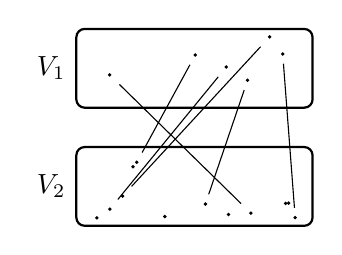
\begin{tikzpicture}[color=black]

\node (rect) at (0,0)[draw,thick,minimum width=3cm, minimum height = 1cm, rounded corners=3pt,label=left:$V_2$]{};

\node (rect2) at (0,1.5)[draw,thick,minimum width=3cm, minimum height = 1cm, rounded corners=3pt,label=left:$V_1$]{};

\pgfmathsetseed{2}
% \def\z{rand}
\foreach \x in {1,...,6}
{
\filldraw (rand*1.4,rand*.4) circle (0.4pt) node(a\x){};
\filldraw (rand*1.4,1.5+rand*.4) circle (0.4pt) node(b\x){};
}

%some extra nodes in the bottom one
\foreach \x in {1,...,6}
{
\filldraw (rand*1.4,rand*.4) circle (0.4pt);
}

\foreach \x in {1,...,6}
{
% \ifthenelse{\x > 1}{\draw[dashed] (a\x) -- (u)}{};
% \foreach \y in {1,...,\x}
% {
\draw (a\x) -- (b\x);
% }
}

\end{tikzpicture}
\end{center}
\caption{Think of elements of $V_1$ as job applicants, and $V_2$ as positions. Then a matching of $V_1$ into $V_2$ is an arrangement so that every job applicant has a position, but some positions could be unfilled.  \label{fig:bipartite_matching}}
\end{marginfigure}


\item[Neighborhood:] For $S\subset V_1$, define the \defn{neighborhood}[graph!neighborhood] $N(S)$ as the set of verticies adjacent to at least one vertex in $S$.
\end{itemize}
The following result\sidenote{\cite{Hallmarriage}} connects these ideas.
\begin{theorem}[Hall's marriage theorem]
Let $G$ be a bipartite graph with bipartition $(V_1,V_2)$. Then $G$ contains a matching of $V_1$ into $V_2$ if and only if 
\begin{equation}	 \label{eq:Hall_condition}
|N(S)| \geq |S| \text{ for every } S\subset V_1. \tag{Hall's condition}
\end{equation}
\end{theorem}
\begin{proof}	
The condition is necessary because you need to have enough verticies available in $N(S)$ for elements of $S$ to match into. We will prove sufficiency by induction on $|V_1|$. The base case is immediate. For the induction step, we will split into two cases.
\begin{enumerate}[{Case }1:]
	\item For every $S\subset V_1$ with $S\neq \emptyset$ and $S\neq V_1$, we have that $|N(S)| > |S|$. 
% \end{enumerate}
In this case, choose  $v\in V_1$; then $v$ has a $w\in V_2$ adjacent to it, because $|N(\{v\})|> |\{v\}|=1$. Apply the induction hypothesis to $G \setminus \{v,w\}$.

We then just need to check Hall's condition on $G' =G \setminus \{v,w\}$. For every $S\subset V_1 \setminus\{v\}$, we have 
\[	
 |N'(S)| \geq |N(S)| -1 \geq |S|,
\]
 where $N'$ is the neighborhood with respect to $G'$. The first inequality holds because we removed at most one neighbor by removing $w$. The second inequality holds from our assumption in this case. Then the induction hypothesis yields a matching on $V_1\setminus \{v\}$ into $V_2\setminus \{w\}$, which we can extend to a matching on $V_1$ into $V_2$ by matching $v$ to $w$.
% \begin{enumerate}[{Case }1:]\setcounter{enumi}{1}
\item There exists $S\subset V_1$ with $S\neq \emptyset$ and $S\neq V_1$, such that $|N(S)| = |S|$. 
% \end{enumerate}
By induction hypothesis,  there exists a matching $M_1$ of $S$ into $N(S)$.

 It remains to find a matching from $V_1\setminus S$ into $V_2 \setminus N(S)$. By induction hypothesis, it is enough to show that for every $T\subset V_1\setminus S$, we have
\[
 |N(T)\cap (V_2 \setminus N(S))| \geq |T|.
\]
 \marginnote{Here's the trick.}Since $S\cup T\subset V_1$, by assumption, we have Hall's condition
\[
 |N(S\cup T)|\geq |S\cup T| = |S| + |T|.
\]

 We know $N(S\cup T) = N(S) \cup N(T) = N(S) \cup (N(T)\setminus N(S))$. So $|N(S\cup T)| = |N(S)| + |N(T)\setminus N(S)| $. So Hall's condition becomes
\[
 |N(T)\setminus N(S)| \geq |T|
\]
 as desired.\qedhere
 \end{enumerate}
\end{proof}


Let's employ Hall's theorem to represent sets. Let 
\[
 \F = \{A_1,A_2,\dotsc,A_m\}
 \] be a set system.
% \begin{definition}
A \defn{system of distinct representatives} for $\F$ is a collection $\{x_1,\dotsc,x_m\}$ of elements such that $x_1,\dotsc, x_m$ are pairwise distinct, and $x_i \in A_i$ for $i\in[m]$.
% \end{definition}
Given $\F$, one can consider the bipartite graph $G$ with bipartition $(V_1,V_2)$ such that $V_1 = \F$ and $V_2= \bigcup_{i\in[m]} A_i$. We join $A_i$ to $x$ iff $x\in A_i$.
Then a system of distinct representatives for $\F$ is exactly a matching on $G$ from $V_1$ into $V_2$. Hall's theorem then immediately implies the following result.
\begin{corollary}
A set system $\F = \{A_1,\dotsc,A_m\}$ has a system of distinct representatives if and only if for every $\F'\subset \F$, 
\[
|\F'| \leq \left|\bigcup_{A\in \F'}A\right|.
\]
\end{corollary}
\newthought{Given a set $X$}, there is a natural bipartite graph and matching which will prove useful.
\begin{corollary} \label{cor:Xr_matching_exists}
Let $X$ be a set with $|X|=n$. Let $G$ be a bipartite graph with bipartition $(X^{(r)}, X^{(r-1)})$ such that $A\in X^{(r)}$ is adjacent to $B \in X^{(r-1)}$ if $B\subset A$. Then if  $r> n/2$, the graph $G$ has a matching of $X^{(r)}$ into $X^{(r-1)}$.
\begin{marginfigure}
\begin{center}
 \begin{tikzcd}[column sep=tiny]
X^{(3)}  & &\{1,2,3\}  \\
X^{(2)} &\{1,2\} \arrow[dash,green]{d}  \arrow[dash]{rd}& \{1,3\} \arrow[dash]{ld}\arrow[dash]{d} \arrow[dash,green]{rd} & \arrow[dash,green]{ld} \arrow[dash]{d}\{2,3\} \\
X^{(1)} & \{1\}  & \{2\} &\{3\} \\
X^{(0)} & & \emptyset
\end{tikzcd}
\end{center}
\caption{Example of the graph relation on $G= (X^{(2)}, X^{(3)})$, with a matching highlighted in green.}
\end{marginfigure}
\end{corollary}
\begin{remark}
This corollory implicitly shows ${n \choose r} \leq {n \choose r-1}$ if $r> n/2$.
\end{remark}
\begin{proof}	
It suffices to check \ref{eq:Hall_condition}. For every $\A\subset X^{(r)}$, we want $|N(\A)| \geq |\A|$. Label
\[
\B:= N(\A) = \{B\in X^{(r-1)}: B\subset A, \text{ for some }A\in \A\}.
\]
Every element of $X^{(r)}$ is incident to $r$ edges of $G$\sidenote{Each edge corresponds to taking an element away from the set.}. So we have $|\A|r$ edges leaving $\A$, ending in $\B$.
Every element of $X^{(r-1)}$ is incident to $n-r+1$ edges of $G$, which can be seen by the fact that there are $n-(r-1)$ possible elements to add to a set $B\in X^{(r-1)}$ to obtain a superset in $X^{(r)}$. So we have at most $|\B|(n-r+1)$ edges leaving $\B$, ending in $\A$\sidenote{Since not every edge leaving $\B$ needs to reach something in $\A$ (it could reach something in $X^{(r)} \setminus \A$), it is only ``at most.''}.
So $|\A|r \leq |\B|(n-r+1)$. But by assumption $r \geq (n-r+1)$, so $|\B| \geq |\A|$ as desired.
\end{proof}

\lect{1}{13}
% \marginnote{Lecture 3: Wednesday, January 13, 2016.}

Recall that $\F\subset \P(X)$ is a \emph{Sperner system} if for all $A,B\in \F$, if $A\leq B$, then $A=B$.
We wish to find $\max |\F|$ such that $\F$ is a Sperner system, as a function $|X| = n$. Note that $X^{(r)}$ is always Sperner, and $|X^{(r)}| = {|X| \choose r}$, which is maximized when $r = \floor{n/2}$.
\begin{theorem}[\cite{sperner1928}] \label{thm:sperner}
If $\F\subset \P(X)$ is Sperner, then $|\F| \leq {n \choose \floor{n/2}}$, where $n=|X|$.
\end{theorem}
\begin{proof}	
\marginnote{A Sperner system is a system of sets such that no two are comparable. A dual notion is a system of sets such that all are comparable. }
An ordered collection $(A_1,A_2,\dotsc, A_k)$ of sets  in $\P(X)$  is a \defn{chain} if $A_1\subsetneqq A_2 \subsetneqq A_3 \subsetneqq\dotsm \subsetneqq A_k$. 
\begin{marginfigure}
\begin{center}
 \begin{tikzcd}[column sep=tiny]
X^{(3)}  & &\{1,2,3\} \arrow[dash]{d}\arrow[dash]{rd}\arrow[dash,green]{ld} \\
X^{(2)} &\{1,2\} \arrow[dash,green]{d}  \arrow[dash]{rd}& \{1,3\} \arrow[dash]{ld}\arrow[dash]{d} \arrow[dash,blue]{rd} & \arrow[dash,red]{ld} \arrow[dash]{d}\{2,3\} \\
\mathbf{X^{(1)}} & \mathbf{\{1\}} \arrow[dash,green]{rd} & \mathbf{\{2\}} \arrow[dash]{d}&\mathbf{\{3\}}\arrow[dash]{ld} \\
X^{(0)} & & \emptyset
\end{tikzcd}
\end{center}
\caption{Consider $X^{(1)}$, a natural maximal Sperner system. Note that each element of $X^{(1)}$ can form a distinct chain, such as $\emptyset \subsetneqq \{1\} \subsetneqq \{1,2\} \subsetneqq \{1,2,3\}$.}\label{fig:Sperner_chains}
\end{marginfigure}
It is enough to show that $\P(X)$ can be partitioned into ${n \choose \floor{n/2}}$ chains. Indeed, every Sperner system can contain $\leq 1$ element from each chain in the partition; see \cref{fig:Sperner_chains} for an example.
Better yet, we partition $\P(X)$ into chains such that every chain contains an element of $X^{(\floor{n/2})}$. 

Let's begin by partitioning all subsets of $X$ of size $\geq \floor{n/2}$.
We will first do this inductively starting from $X^{(\floor{n/2})}$, and extending the partition to $X^{(\floor{n/2})}\cup X^{(\floor{n/2}+1)}\cup\dotsm \cup X^{(k)}$ to $X^{(k+1)}$ using the matching obtained in \cref{cor:Xr_matching_exists} from $X^{(k)}$ to $X^{(k+1)}$ by adding each element of $X^{(k+1)}$ to the chain of the set it's matched to. Note that are chains are not maximal; some (all but one) truncate before they reach the top, $X^{(n)}$.
Then we can extend the partition to sets of size $< \floor{n/2}$ by symmetry.
\end{proof}
\begin{remark}
This proof is instructive and provides the useful technique of partitioning into chains. But we can prove stronger results with slicker proofs.
\end{remark}
Suppose $k< n/2$ and we want to find the maximum size Sperner system such that every set in the system has size $\leq k$.
As one may guess, the maximum size will be $|X^{(k)}| = {n\choose k}$. To show this, we'll use the following result.
\begin{theorem}[Lubell, Meshalkin, Yamamoto, Boll\'obas, and possibly others, A.K.A. the LYM inequality] \marginnote{\cite{LUBELL_LYM,Meshalkin_LYM,yamamoto1954_LYM,Bollab_LYM}}
\label{thm:LYM_inequality}
Let $\F\subset \P(X)$, $|X|=n$ be a Sperner system.
Let $\F_k = \F\cap X^{(k)}$ be the set of $k$ element sets in $\F$, and let $f_k = |\F_k|$. Then
\begin{equation}	\tag{LYM} 
\label{eq:LYM}
\sum_{k=0}^n \frac{f_k}{{n\choose k}} \leq 1.
\end{equation}
\end{theorem}
\begin{remark}
We have
\[
1 \geq \sum_{k=0}^n \frac{f_k}{{n\choose k}} \geq \sum_{k=0}^n \frac{f_k}{{n\choose \floor{n/2}}},
\]
thus
\[
{n\choose \floor{n/2}} \geq \sum_{k=0}^n f_k = |\F|
\]
which is Sperner's theorem.
\end{remark}
\begin{proof} Let's assume $X=[n]$ for convenience.
Consider all maximum chains in $\P(X)$ and count how many chains an element of $\F$ belongs to. Each of the maximal chains is of the form $\emptyset = A_0$, $A_1$, \ldots, $A_n = X = [n]$, and $|A_i| = i$. So each maximal chain corresponds to an ordering $a_1,a_2,\dotsc,a_n$ of $[n]$, where $\{a_i\} = A_i \setminus A_{i-1}$, is the element you add to $A_i$ to get the next set in the chain.

Thus, there are $n!$ maximal chains (the number of re-orderings of $[n]$). Consider
$F \in X^{(k)}$.
How many  maximal chains is $F$ in? If $k=0,n$, $F$ is in every chain, so $n!$. If $k=1$, then $F$ is in $(n-1)!$ chains. If $k=2$, then $2!(n-2)!$. In general, $F$ is in $k!(n-k)!$ maximal chains\sidenote{We choose $k$ to get to the set, then $(n-k)$ to finish the chain.} Each maximal chain contains $\leq 1$ element of $\F$. The total number of elements of $\F$ in all maximum chains is
\[
 \sum_{k=0}^n f_k k!(n-k)!\leq n!
\]
Dividing by $n!$, we obtain the LYM inequality.
\end{proof}
\begin{remark}
Let's consider an alternate proof. Let $C$ be a uniformly randomly chosen maximal chain, and consider the expectation value of the number of elements of $C\cap \F$. Of course, there is at most 1 element, since $\F$ is a Sperner system. On the other hand,
\begin{align*}	
\E ( | C\cap \F|) &=\sum_{k=0}^n \E( | C \cap \F_k|) = \sum_{k=0}^n f_k \cdot (\text{probability that a set of size $k$ is in $C$})\\
 &=  \sum_{k=0}^n f_k \cdot \frac{1}{(\text{number of sets of size $k$)}} = \sum_{k=0}^n \frac{f_k}{{n \choose k}} \leq 1.
\end{align*}
\end{remark}


When does equality hold in LYM? Certainly when $\F= X^{(r)}$ for any $r$. We'd like to show this condition is necessary as well, but to do so, we'll first prove a more refined inequality in which equality is easier to check. Then we'll use this to show sufficiency for equality in the LYM inequality.

\begin{theorem}[Local LYM inequality] \label{thm:local_LYM}
Let $\A\subset X^{(r)}$, and $|X|=n$. Define
$\partial \A \subset X^{(r-1)}$
the \defn{shadow} of $A$ by
\[
\partial \A := \{B\in X^{(r-1)}: B\supseteq A \text{ for some }A\in \A \}.
\]
Then
\begin{equation}	\label{eq:local_LYM} \tag{Local LYM}
\frac{|\partial \A|}{{n\choose r-1}} \geq \frac{|\A|}{{n \choose r}}
\end{equation}
or equivalently,
\[
 r| \A| \leq |\partial \A| (n-r+1).
\]
Moreover, equality holds if and only if $\A= \emptyset$ or $\A=  X^{(r)}$.
\end{theorem}
\begin{proof}	
\[
 r|\A| = | \{ (B,A): B\in \partial A, \, A\in \A, \, B\subset A\}| \leq |\partial A| (n-r+1)
 \] as seen in \cref{cor:Xr_matching_exists}.
If equality holds, then $\A$ contains all supersets in $X^{(r)}$ of all sets in $\partial A$. 


\begin{marginfigure}
\begin{center}
\begin{tikzcd}[column sep=tiny]
\A & \{x_1,\dotsc,x_r\} \arrow[dash]{d} \arrow[dash]{rd} & \arrow[dash]{ld} \\
\partial \A & \{x_2,\dotsc,x_n\} & \{x_1,x_2,\dotsc,x_n\}
\end{tikzcd}
\end{center}
\caption{If $\A$ contains all supersets in the $X^{(r)}$ layer of sets in the shadow $\partial \A$, then as long as $\A\neq \emptyset$, it must contain every set; here, for example, $\A$ has to include the endpoint of the edge leaving the bottom left vertex. }
\end{marginfigure}

Consider the graph as in \cref{cor:Xr_matching_exists}:  there are no edges from $A\cup \partial A$ to the remaining verticies, so since $G$ is connected\sidenote{as is easy to check},  we have equality in \eqref{eq:local_LYM}.
\end{proof}

\begin{theorem}
The equality in the LYM inequality \eqref{eq:LYM} holds iff $\F = X^{(r)}$ for some $r$.
\end{theorem}
\begin{proof}	
Inductively define $G_n = \F_n$, and for $k < n$, $G_k  = \partial G_{k+1} \cup \F_k$. \marginnote{$G_k$ is the set of all $k$-element sets which are subsets of sets in $\F$.}

Let $\phi_k = \frac{f_k}{{n \choose k}}$ be the proportion of sets of $\F$ in $X^{(k)}$. Similarly, set $\gamma_k = \frac{|G_k|}{{n\choose k}}$. By the local LYM,
\[
\frac{|\partial G_{k+1}|}{{n\choose k}} \geq \frac{|G_{k+1}|}{{n\choose k+1}} = \gamma_{k+1}
\]
So,
\[
\gamma_k = \frac{|\partial G_{k+1} \cup \F_k|}{{n\choose k}} = \frac{|\partial G_{k+1}|}{{n\choose k}} + \frac{|\F_k|}{{n\choose k}} \geq  \gamma_{k+1} + \phi_k
\]
where we are using that $\F$ is Sperner, so that $\partial G_{k+1}$ is disjoint from $\F_k$. Thus, we have $\gamma_k \geq \gamma_{k+1} + \phi_k$, with equality iff $\gamma_{k+1} = 1$ or $\gamma_{k+1} = 0$. \marginnote{Since that is when we have equality in \cref{eq:local_LYM}.}

Note $\gamma_n = \phi_n$. Then
\begin{gather*}	
\gamma_{n-1} \geq \gamma_n + \phi_{n-1} = \phi_n + \phi_{n-1}\\
\gamma_{n-2} \geq \gamma_{n-1} + \phi_{n-2} = \phi_n + \phi_{n-1} + \phi_{n-2}\\
\text{etc.}\\
\gamma_k \geq \phi_n + \phi_{n-1} + \dotsm + \phi_k.
\end{gather*}
Hence, $1 \geq \gamma_0 \geq \phi_n + \phi_{n-1} + \dotsb + \phi_0$. This is the LYM inequality. But equality holds if $\gamma_k = \gamma_{k+1} +\phi_k$ for each $k$, i.e. $\gamma_{k+1} = 1$ or $\gamma_{k+1} = 0$ for each $k$. Assuming we have equality, we use that $\gamma_k$ is non-increasing with $k$, so there must exist $k_0$ such that $\gamma_{k_0} = 1$, and $\gamma_{k_0+1} = 0$ (writing $\gamma_{n+1} = 0$). Thus, there are no sets in $\F$ of size at least $k+1$. In other words, $G_{k+1} = \emptyset$, and $G_k = \F_k = X^{(k)}$. But then we must have $\F  = X^{(k)}$ as desired, since $\F$ may not have any super sets or subsets of $X^{(k)}$, i.e., any other set in $\P(X)$.
\end{proof}
\begin{remark}
The matchings with $X^{(r)}$ and $X^{(r-1)}$ are the essential objects here in proving the local LYM, and hence LYM and its equality.
\end{remark}
\begin{exercise}
Prove Sperner's theorem using the original way: partitioning into ${n\choose \floor{n/2}}$ chains by induction on $n$ instead of Hall's theorem.
\marginnote{This is \cref{thm:sym_part}.}
\end{exercise}

